\documentclass[]{article}
\usepackage[utf8]{inputenc}
\usepackage{polski}
\usepackage{graphicx}
\graphicspath{ {./images/} }
\usepackage[margin=0.5in]{geometry}
\usepackage{gensymb}
\usepackage{textcomp}
\usepackage{siunitx}
\usepackage{float}

\begin{document}

\begin{figure}[tp!]
	\center{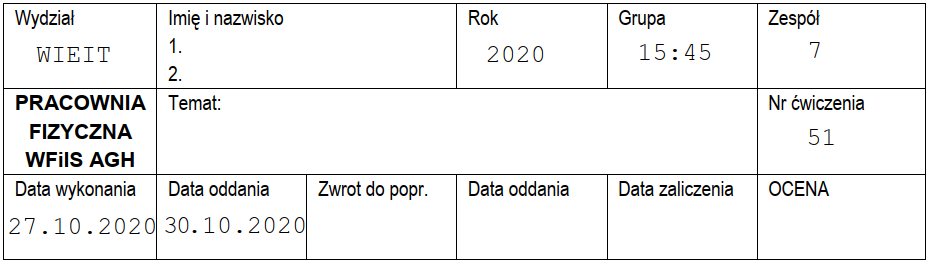
\includegraphics{F}}
\end{figure}

\begin{center}
	\section*{Współczynnik załamania światła dla ciał stałych }
	\emph{Dzmitry Mikialevich}
\end{center}
\begin{center}
	\emph{Wojciech Sikora}
\end{center}
\tableofcontents
\newpage

\section{Wstęp}

\subsection{Cel ćwiczenia}
Wyznaczenie współczynnika załamania światła dla płytki szklanej i pleksiglasowej metodą
pomiaru grubości pozornej płytki przy pomocy mikroskopu. 

    
\subsection{Opis ćwiczenia}
Zestawione wyniki opierają się na równaniu określającym zależność pomiędzy współczynnikiem załamania, oznaczonym jako \(n\), od rzeczywistej grubości płytki \(d\) i pozornej grubości płytki \(h\).
\[n =\frac{d}{h}\] \
Pozorną grubość płytki h wyznaczamy mierząc przesunięcie tubusa mikroskopu między położeniami ostrego widzenia
kresek umieszczonych na obu powierzchniach płytki. 

    
\section{Układ Pomiarowy}
W skład układu pomiarowego weszły następujące elementy:
\newline

1. Mikroskop wyposażony w czujnik mikrometryczny i nasadkę krzyżową. 


2. Śruba mikrometryczna.


3. Jedna płytka ze szkła i dwie płytki z pleksiglasu różnej grubości.

\newline
\newline


\begin{figure}[h]
	\center{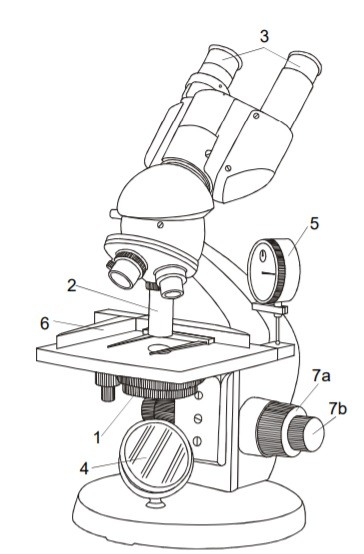
\includegraphics{mikroskop}}
	\textbf{\caption{Mikroskop}}
	
\end{figure}

Mikroskop i jego elementy: 1 – kondensor, 2 – obiektyw, 3 – okular, 4 – lusterko lub lampka oświetleniowa, 5 – czujnik mikrometryczny, którego
stopka spoczywa na ruchomej części mikroskopu, 6 – nasadka krzyżowa XY mocująca z pokrętłami do przesuwu płytki, 7a – pokrętło służące do przesuwu stolika ruchem zgrubnym, 7b –
pokrętło służące do przesuwu stolika ruchem dokładnym






\section{Przebieg doświadczenia}
W  ramach  doświadczenia  przeprowadziliśmy kilka serii pomiarów dla trzech różnych płytek: jednej szklanej i dwóch pleksiglasowych z kreskami na każdej ze stron. Dla każdej płytki mierzyliśmy odległość od dolnej i górnej kreski, dzięki czemu obliczyliśmy grubość pozorną. Uzyskaliśmy średnią wartość grubości pozornej, która pozwoliła ustalić wartość współczynnika załamania.




\section{Wyniki Pomiarów}


	\begin{table}[h]
		\centering
		\begin{tabular}{|l|l|l|l|}
			\hline
                lp. & \begin{tabular}{@{}c@{}}Dolna odległość \\ \(a_d\) [mm]\end{tabular}  & \begin{tabular}{@{}c@{}}Dolna odległość \\ \(a_g\) [mm]\end{tabular}  & \begin{tabular}{@{}c@{}}Grubość pozorna  \\\(h=a_d-a_g\:[mm]\)\end{tabular}  \\ \hline
                1 & 7,61 & 4,44 & 3,17  \\ \hline 
                2 & 7,58 & 4,39 & 3,19  \\ \hline
                3 & 7,65 & 4,41 & 3,24  \\ \hline
                4 & 7,55 & 4,41 & 3,14  \\ \hline
                \\ \hline
                & \multicolumn{2}{|c|}{Średnia grubość pozorna h:} & 3,185 \\ \hline
                & \multicolumn{2}{|c|}{Niepewność grubości pozornej u(h):} & 0,022 \\ \hline
                & \multicolumn{2}{|c|}{Grubość rzeczewista d: } & 4,86 \\ \hline
                & \multicolumn{2}{|c|}{Niepewność grubości rzeczewistej u(d): } & 0,01 \\ \hline
                
			
		\end{tabular}
		\textbf{\caption{Wskazanie czujnika dla szkła}
		}
	\end{table}
	
	
		\begin{table}[h]
		\centering
		\begin{tabular}{|l|l|l|l|}
			\hline
                lp. & \begin{tabular}{@{}c@{}}Dolna odległość \\ \(a_d\) [mm]\end{tabular}  & \begin{tabular}{@{}c@{}}Dolna odległość \\ \(a_g\) [mm]\end{tabular}  & \begin{tabular}{@{}c@{}}Grubość pozorna  \\\(h=a_d-a_g\:[mm]\)\end{tabular}  \\ \hline
                1 & 7,82 & 5,34 & 2,48 \\ \hline
                2 & 7,86 & 5,32 & 2,54 \\ \hline
                3 & 7,84 & 5,35 & 2,49 \\ \hline   
                \\ \hline
                & \multicolumn{2}{|c|}{Średnia grubość pozorna h:} & 2,5 \\ \hline
                & \multicolumn{2}{|c|}{Niepewność grubości pozornej u(h):} & 0,019 \\ \hline
                & \multicolumn{2}{|c|}{Grubość rzeczewista d: } & 3,86 \\ \hline
                & \multicolumn{2}{|c|}{Niepewność grubości rzeczewistej u(d): } & 0,01 \\ \hline
			
		\end{tabular}
		\textbf{\caption{Wskazanie czujnika dla Pleksiglasa 1 }
		}
	\end{table}
	
			\begin{table}[h]
		\centering
		\begin{tabular}{|l|l|l|l|}
			\hline
                lp. & \begin{tabular}{@{}c@{}}Dolna odległość \\ \(a_d\) [mm]\end{tabular}  & \begin{tabular}{@{}c@{}}Dolna odległość \\ \(a_g\) [mm]\end{tabular}  & \begin{tabular}{@{}c@{}}Grubość pozorna  \\\(h=a_d-a_g\:[mm]\)\end{tabular}  \\ \hline
                1 & 8,55 & 7,25 & 1,3 \\ \hline
                2 & 8,64 & 7,29 & 1,35 \\ \hline
                3 & 8,61 & 7,34 & 1,27 \\ \hline
                4 & 8,62 & 7,37 & 1,25 \\ \hline
                5 & 8,62 & 7,22 & 1,4 \\ \hline
                6 & 8,64 & 7,32 & 1,32 \\ \hline
                7 & 8,62 & 7,3 & 1,32 \\ \hline
                \\ \hline
			    & \multicolumn{2}{|c|}{Średnia grubość pozorna h:} & 1,31 \\ \hline
			    & \multicolumn{2}{|c|}{Niepewność grubości pozornej u(h):} & 0,019 \\ \hline
                & \multicolumn{2}{|c|}{Grubość rzeczewista d: } & 1,94 \\ \hline
                & \multicolumn{2}{|c|}{Niepewność grubości rzeczewistej u(d): } & 0,01 \\ \hline
		\end{tabular}
		\textbf{\caption{Wskazanie czujnika dla Pleksiglasa 2}
		}
	\end{table}
\newline


\section{Opracowanie wyników Pomiarów}

    \subsection{Współczynnik załamania \mathbf{n} dla każdej badanej płytki}
    Współczynnik załamania dla szkła:
    \[n_{szk}=\frac{d}{h}=\frac{4,86}{3,185}=1,53\]
    
    Współczynnik załamania dla pleksiglasu 1:
    \[n_{pleks1}=\frac{d}{h}=\frac{3,86}{2,5}=1,54\] 
    
    Współczynnik załamania dla pleksiglasu 2:
    \[n_{pleks2}=\frac{d}{h}=\frac{1,94}{1,31}=1,48\] 


\subsection{Niepewność typu B i typu A}

Grubość rzeczywista każdej z płytek była mierzona za pomocą śruby mikrometrycznej, niepewność 
typu B (graniczną) dla której przyjęliśmy jako \(u_g(d) = 0,01\: mm\), wtedy niepewność standardowa wynosi \(u_{st}(d) = \frac{0,01}{\sqrt{3}}= 0,0058\:mm\).\newline
Niepewność typu A dla grubości pozornej h szkła:
\[u(h_{szk}) = \sqrt{\frac{\sum (h_i - h_{śr})^2}{n(n-1)}} = 0,022\:mm\]
Niepewność typu A dla grubości pozornej h Pleksiglasa 1:
\[u(h_{pleks1}) = \sqrt{\frac{\sum (h_i - h_{śr})^2}{n(n-1)}} = 0,019\:mm\]
Niepewność typu A dla grubości pozornej h Pleksiglasa 2:
\[u(h_{pleks2}) = \sqrt{\frac{\sum (h_i - h_{śr})^2}{n(n-1)}} = 0,019\:mm\]

\subsection{Niepewność złożona współczynnika załamania}
Niepewność złożona współczynnika załamania z prawa przenoszenia niepewności:

\[u(n)=\sqrt{[\frac{1}{h}u(d)]^2+[\frac{-d}{h^2}u(h)]^2}\]
\[u(n_{szk})=0,011\]
\[u(n_{pleks1})= 0,013\]
\[u(n_{pleks2})=0,023\]

Niepewność złożona współczynnika załamania z prawa przenoszenia niepewności względnych:

\[\frac{u(n)}{n}=\sqrt{[\frac{u(d)}{d})]^2+[\frac{u(h)}{h}]^2}\]
czyli
\[u(n)=n\sqrt{[\frac{u(d)}{d})]^2+[\frac{u(h)}{h}]^2}\]
\[u(n_{szk})=0,011\]
\[u(n_{pleks1})= 0,013\]
\[u(n_{pleks2})=0,023\]





\subsection{Zestawienie wyników}
	\begin{table}[H]
		\centering
		\begin{tabular}{|l|l|l|l|l|}
			\hline
                Rodzaj materiału & Zmierzone n  & Niepewność u(n) & Tablicowe n  & Różnica \(\Delta n\)\\ \hline
                Szkło & 1,53 & 0,011 & 1,5 & 0,03 \\ \hline
                Pleksiglas 1 (Grubszy) & 1,54  & 0,013 & 1.489 &  0,045\\ \hline
		    	Pleksiglas 2 (Cieńszy) & 1,48  & 0,019 & 1.495 & 0,015\\ \hline
		\end{tabular}
		\textbf{\caption{Zestawienie wyników}
		}
	\end{table}
\subsection{Wnioski}
\begin{itemize}
		\item Obliczyliśmy współczynniki załamania dla różnych płytek ze średnią niepewnością \(u_{sr}(n) = 0,016\), co pozwala uważać doświadczenie za wykonane poprawnie.
		\item  Różnicy między wartościami tablicowymi (wziętymi dla długości fali równej 560 nm) a otrzymanymi z doświadczenia za wyjątkiem pleksiglasu 1 (z powodu niedużej ilości wykonanych dla niego doświadczeń) mieszczą się w niepewności, co pokazuję wysoką precyzję wykonanego doświadczenia.
	\end{itemize}
\end{document}